\chapter{Data Analysis}

For the gene expression data set previously described in Section~\ref{data}, we
applied the TMLE-based biomarker evaluation procedure to obtain separate,
individual estimates of the association of each of the roughly $22,000$
biomarkers with benzene exposure, while controlling for potential confounding
based on age, sex, and smoking status. The values obtained from applying this
procedure on a biomarker-by-biomarker basis correspond to the contributions of
each potential biomarker to changes measured by the ATE (the target parameter of
interest, in this case), based on the influence curve decomposition of the ATE
parameter. While having a direct interpretation in relation to the ATE, such
transformed expression values hold little bearing on statistical inference.

Using the ATE, the moderated t-statistic for the test performed is as follows:

$$
\tilde{t}_b = \frac{\sqrt{n}(\Psi_{b,n}(P_n^*))}{\tilde{s}_{b,n}}
,$$
where $\tilde{s}_{b,n}^2=\frac{d_0s_0^2+d_b (s_b^2(IC_{b,n}))}{d_0+d_b},$ where
$d_b$ is the degrees of freedom for the $b^{th}$ biomarker, $d_0$ is the degrees
of freedom for the remaining biomarkers, $s_b(IC_{b,n})$ the standard deviation
for the $b^{th}$ biomarker, and $s_0$ the common standard deviation across all
biomarkers towards which the empirical Bayes procedure performs shrinkage.

In order to isolate a set of differentially up-regulated or down-regulated
biomarkers, we apply the moderated t-statistic ~\cite{smyth2004linear} to test
for group differences based on the observed benzene exposure status. This
results in a table including the moderated t-statistic for each test of the
ATE-transformed values between the exposed and unexposed groups (a coefficient
corresponding to exposure in the gene-wise linear models fit via the approach of
``limma''), standard errors of the coefficient, raw p-values, and adjusted
p-values from application of the Benjamini-Hochberg procedure for controlling
the FDR~\cite{benjamini1995controlling}. See table~\ref{table:topresults} below:

% latex table generated in R 3.3.2 by xtable 1.8-2 package
% Fri Mar  3 14:28:32 2017
\begin{table}[H]
\centering
\label{table:topresults}
\begin{tabular}{rlrrr}
  \hline
  & Biomarker ID & ATE Change & p-value & adjusted p-value \\
  \hline
  1 & 198 & 1.69167E+01 & 1.04812E-54 & 2.90551E-51 \\
  2 & 1055 & 8.30585E+00 & 1.73105E-47 & 1.74498E-44 \\
  3 & 1764 & -1.83308E+00 & 6.00103E-55 & 1.90121E-51 \\
  4 & 2469 & 1.70375E+02 & 2.87168E-47 & 2.76893E-44 \\
  5 & 3607 & -4.36856E+00 & 6.07654E-47 & 5.39038E-44 \\
  6 & 4195 & 7.19651E+00 & 1.38153E-52 & 2.78529E-49 \\
  7 & 6207 & -3.05520E+01 & 1.17986E-57 & 5.23316E-54 \\
  8 & 6262 & -1.30293E+01 & 8.96437E-49 & 1.10446E-45 \\
  9 & 7481 & -2.72348E+01 & 1.06992E-48 & 1.24883E-45 \\
  10 & 8664 & -9.94950E+01 & 3.25553E-47 & 3.00824E-44 \\
  11 & 10255 & 1.07510E+01 & 9.07492E-54 & 2.01255E-50 \\
  12 & 11073 & -2.88118E+01 & 7.45674E-54 & 1.83742E-50 \\
  13 & 12898 & -2.50923E+01 & 1.34871E-58 & 7.47759E-55 \\
  14 & 14003 & -1.84590E+01 & 5.86475E-59 & 4.33542E-55 \\
  15 & 14472 & 7.39674E-01 & 2.61339E-52 & 4.82976E-49 \\
  16 & 16255 & -3.41521E+01 & 1.31512E-50 & 2.08324E-47 \\
  17 & 16454 & -5.35507E+00 & 8.58888E-48 & 9.52378E-45 \\
  18 & 16608 & -3.34112E+00 & 1.16964E-55 & 4.32320E-52 \\
  19 & 16658 & -6.27276E+00 & 2.21905E-51 & 3.78552E-48 \\
  20 & 17537 & -1.77342E+02 & 2.27910E-59 & 2.52718E-55 \\
  21 & 17982 & -1.09417E+02 & 4.52028E-63 & 1.00246E-58 \\
  22 & 18337 & 1.49518E+00 & 1.87252E-49 & 2.44275E-46 \\
  23 & 19399 & -1.06334E+02 & 3.36332E-50 & 4.97256E-47 \\
  24 & 20294 & -1.16305E+02 & 1.64737E-47 & 1.73970E-44 \\
  25 & 22058 & -1.13907E+01 & 6.07700E-50 & 8.42310E-47 \\
  \hline
\end{tabular}
\caption{The top $25$ biomarkers isolated as a result of applying the moderated
  t-statistic to the ATE parameter. Applying empirical Bayes moderation to the
  variance of the ATE estimates produced by standard TMLE-based procedures
  identifies nearly $5,000$ biomarkers as significant in total.}
\end{table}

The analysis presented can be completely replicated by using the ``biotmle''
software package, which provides facilities for visualizing the results. Using
this R package, a heatmap for visualizing differences in the ATE induced by
benzene exposure, with all $125$ subjects on the x-axis and the top $25$
isolated biomarkers on the y-axis, may be produced. The heatmap, created using
the ``superheat'' R package \cite{barter2017superheat}, is displayed as
figure~\ref{fig:heatmap} below:

\begin{figure}[H]
  \vspace{-4em}
  \label{fig:heatmap}
  \centering
  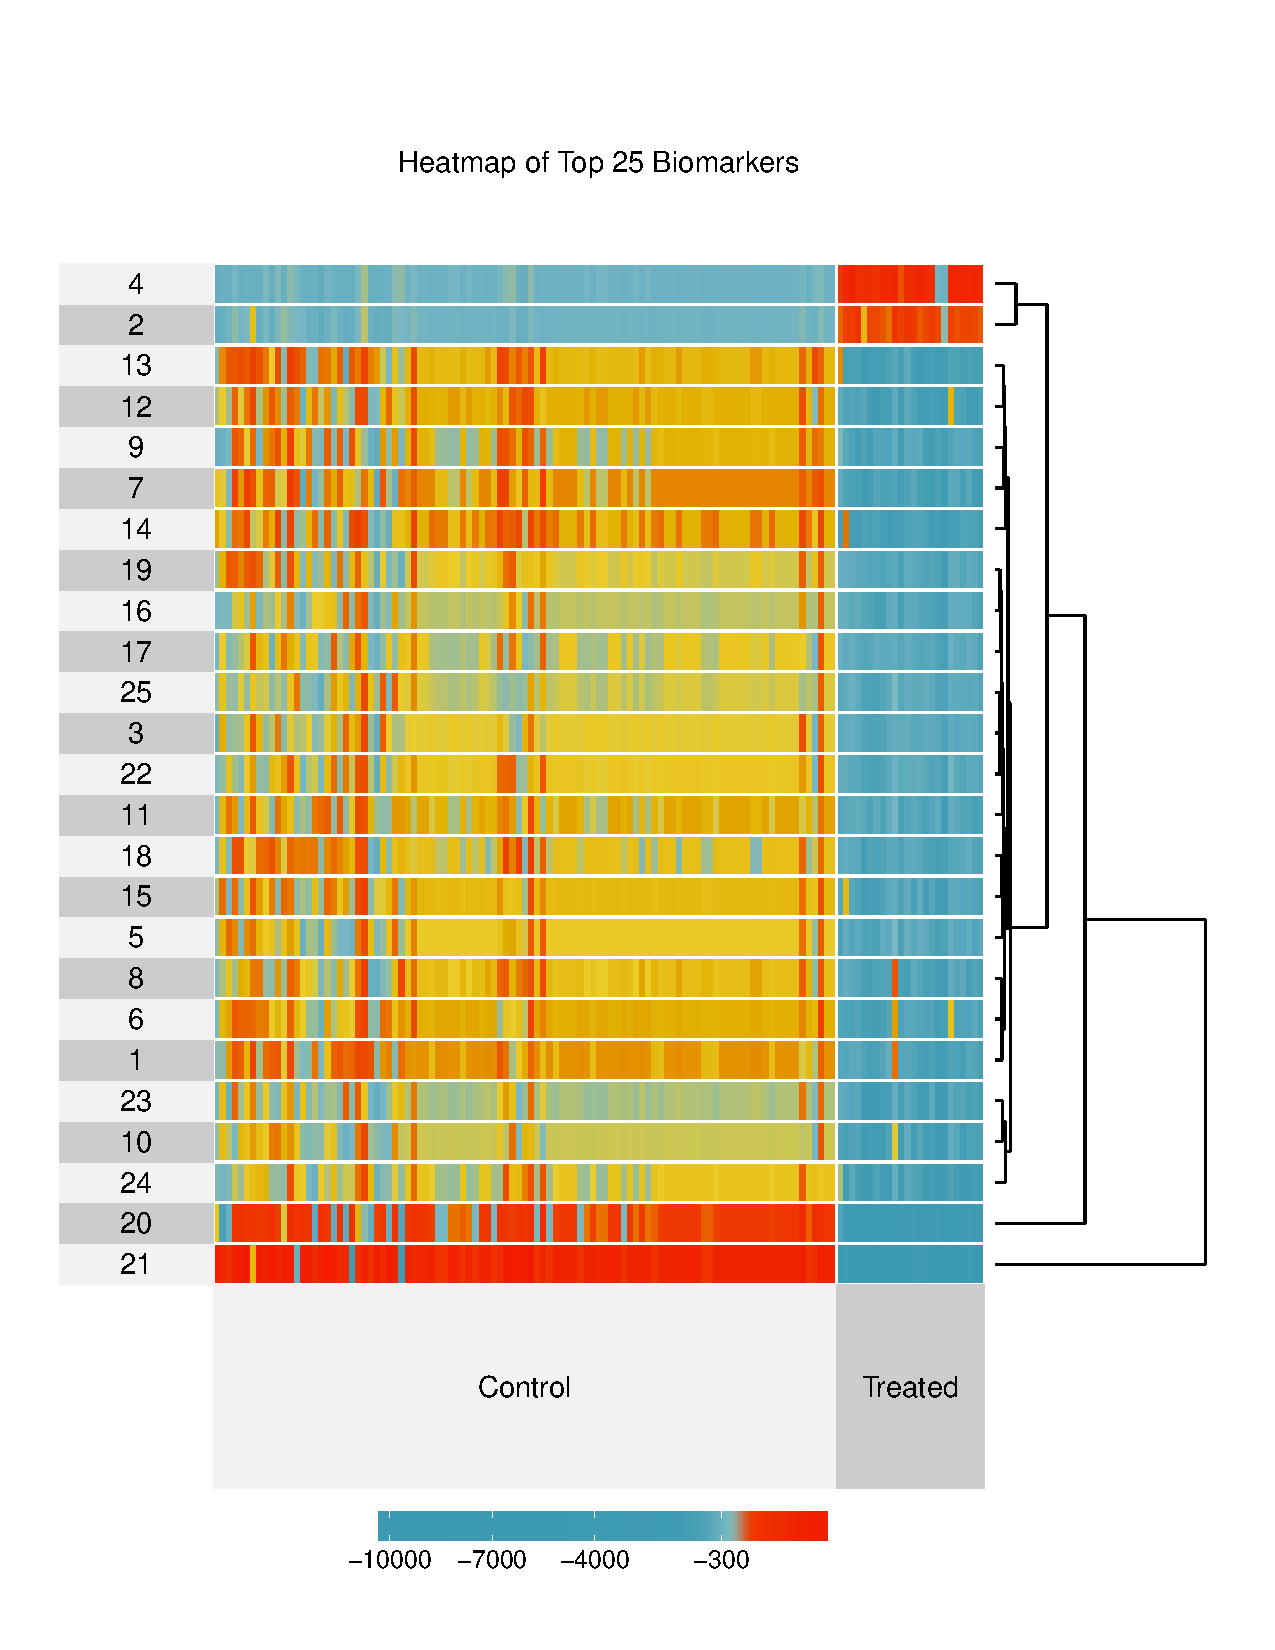
\includegraphics[scale=0.75]{figs/superheatmap.pdf}
  \caption{Heatmap of the ATE estimates. Blue indicates a depression in the
    ATE, while red indicates elevation of the ATE, based on exposure to the
    maximal level of benzene as opposed to the minimal level. Hierarchical
    clustering is performed on the top $25$ biomarkers identified by the
    proposed procedure.}
\end{figure}

As expected, the use of moderated statistics reduces the spread of the standard
deviation estimates of the influence curve by probe ($\tilde{s}^2_b$) across the
approximately $20,000$ probes, and the corresponding Wald statistics for testing
the target parameter, in comparison to using the original standard error. The
results of our analysis indicate that application of moderated statistics to
asymptotically linear parameters constitutes a powerful approach for assessing
variable importance, based on treatment or exposure, in the context of
high-dimensional investigations of biomarkers. We conclude that using this
adaptation of TMLE, complimented by moderated statistics implemented in the
``limma'' R package, reduces the variability of standard errors and reduces the
number of probes identified as significant, leading to more stable and robust
inference, while providing the opportunity to evaluate biomarkers in the context
of statistical parameters of scientific relevance, such as the average treatment
effect focused on in the example discussed above.
